\chapter{The Kiss Experiment and What Statistics Is For}
\label{ch:kiss}

\begin{chaptergoals}
\begin{itemize}[nosep]
\item Probability and statistics as the same picture read in opposite directions: from a known truth to the data it will produce, and from observed data back to the truths that could have produced it.
\item The book's running example, the kiss experiment, and the three modeling assumptions that turn $80$ out of $124$ into a mathematical problem.
\item Why the sample proportion is a random variable, what population it is a sample from, and the three questions about it that the next chapters answer.
\item The trinity of statistical inference: estimation, confidence intervals and hypothesis testing, each stated for the kiss experiment and each pointed to the chapter that delivers it.
\end{itemize}
\end{chaptergoals}

\section{Probability and statistics are the same picture read in opposite directions}
\label{sec:kiss-dogma}

Probability studies randomness.
Sometimes the physical process is completely known: dice, cards, roulette, fair coins.
Roll one die.
Alice gets \$1 if the number of dots is at most $3$; Bob gets \$2 if the number of dots is at most $2$.
Who would you rather be?
You don't need any data to answer: Alice expects $1 \times \frac{3}{6} = \$0.50$ per roll, Bob expects $2 \times \frac{2}{6} \approx \$0.67$, so Bob.
Roll two dice and win \$100 if you called the sum correctly: you call $7$ because six of the thirty-six equally likely outcomes sum to $7$ and no other total has as many.
In both cases the mechanism is known, and probability deduces what the data will look like.

Statistics is the reverse problem.
The mechanism is unknown, you observe data it produced, and you want to say something about the mechanism.
The two directions fit into a single diagram, the central dogma of probability and statistics.

\begin{center}
\begin{tikzpicture}[
  box/.style={draw, rounded corners=3pt, minimum width=3.2cm, minimum height=1.0cm, align=center, font=\small, fill=gray!5},
  arr/.style={-{Latex[length=2.5mm]}, thick}
]
  \node[box] (truth) {Truth\\ \scriptsize the mechanism, $p$};
  \node[box, right=4.2cm of truth] (data) {Observations\\ \scriptsize the data, $80$ of $124$};
  \draw[arr, boxblue!80!black] ([yshift=4pt]truth.east) -- node[above, font=\small] {Probability} ([yshift=4pt]data.west);
  \draw[arr, boxorange!80!black] ([yshift=-4pt]data.west) -- node[below, font=\small] {Statistics} ([yshift=-4pt]truth.east);
\end{tikzpicture}
\end{center}

A drug trial shows both directions at work.
\textit{Probability:} previous studies showed the drug to be $80\%$ effective.
Then in a study of $100$ patients you can anticipate that on average $80$ will be cured, and that at least $65$ will be cured with probability $99.99\%$.
\textit{Statistics:} you observe that $78$ of $100$ patients were cured.
You will be able to conclude, by the end of \cref{ch:confidence-intervals}, that you are $95\%$ confident the drug is effective on between $69.9\%$ and $86.1\%$ of patients.
(That sentence is the standard shorthand for a confidence interval; \cref{sec:ci-meaning} says exactly what it does and does not claim.)
\Cref{fig:probstat} draws both halves.

\begin{figure}[htbp]
\centering
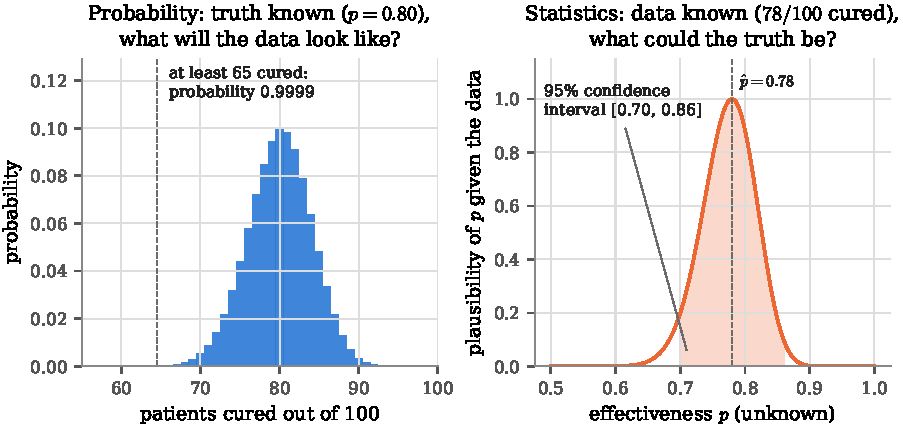
\includegraphics[width=\textwidth]{fig_probability_vs_statistics}
\caption{The drug example in both directions. Left, probability: the effectiveness $p = 0.80$ is known, so the number cured out of $100$ has a known distribution (Binomial), and the probability of at least $65$ cures is a computable $0.9999$. Right, statistics: $78$ of $100$ were cured and $p$ is unknown; the curve shows how plausible each value of $p$ makes the data (it is the likelihood of \cref{ch:likelihood}, scaled to peak at $1$), and the shaded band is the $95\%$ confidence interval $[0.70, 0.86]$ of \cref{ch:confidence-intervals}.}
\label{fig:probstat}
\end{figure}

Notice what the right-hand panel is \textit{not}.
It isn't a probability distribution for $p$: in this book $p$ is a fixed unknown number, not a random variable, and the curve is a plausibility ranking of candidate truths, not a density.
The one place where $p$ does get a distribution is \cref{ch:bayes-intro}, and the difference is the whole point of that chapter.

\begin{bridge}[descriptive and inferential statistics]
An introductory course divides statistics into descriptive (summarize the data you have) and inferential (say something about the population you don't have).
This book is entirely about the second, and it adds the step the introductory course leaves implicit: a mathematical model of how the data were produced, precise enough that the inferential statements can be proved rather than asserted.
The model is the thing on the left of the diagram, and every method in the book is a way of traveling the orange arrow with a guarantee attached.
\end{bridge}

\section{The kiss experiment}
\label{sec:kiss-test}

Newborn babies, lying on their backs, turn their heads to the right more often than to the left.
A 2003 paper in \textit{Nature} asked whether that preference survives into adulthood, and looked for it in an unexpected place: which way couples turn their heads when they kiss.\footnote{O.~G\"unt\"urk\"un, `Adult persistence of head-turning asymmetry', \textit{Nature} 421 (2003), 711.}
The author watched kissing couples in public places (airports, train stations, beaches and parks) in the United States, Germany and Turkey, and recorded for each couple which way their heads turned.

Let $p$ denote the proportion of couples who turn their heads to the right when kissing.
The statistical experiment: observe $n$ kissing couples and record each outcome, $1$ for right and $0$ for left.
Estimate $p$ with the proportion $\hat{p}$ of couples who turned right.
Of the $n = 124$ couples observed, $80$ turned to the right, so
\[
\hat{p} = \frac{80}{124} = 64.5\%.
\]

Two things about the number $124$ because the whole book turns on them.
It is small, and it is small for a reason: each observation needs an observer in a public place at the right moment, close enough to see which way the heads turn, and a kiss is over in seconds.
And it is the only sample there is: the study is published, and the question is what these $124$ observations can be made to say.
Everything that follows is about how much a sample of this size can be made to say.

Now some random intuition.
$64.5\%$ is much larger than $50\%$, so there seems to be a preference for turning right.
But suppose the data had been right, right, left, that is $n = 3$: that's $66.7\%$ to the right, an even bigger number.
Better evidence?
Obviously not; intuitively you need a large enough sample size to make a call.
How large?
Another way to put the problem: for $n = 124$, what is the minimum number of couples turning right that you would need to see to be convinced that $p > 50\%$?
$63$? $72$? $75$? $80$?
Mathematical modeling is needed to understand the accuracy of this procedure, and the number turns out to be $72$ (\cref{sec:kiss-trinity}).

\section{Modeling assumptions}
\label{sec:kiss-assumptions}

Formally, the procedure consists of the following.
For $i = 1, \ldots, n$, define $R_i = 1$ if the $i$-th couple turns to the right and $R_i = 0$ otherwise.
The estimator of $p$ is the sample average
\[
\hat{p} = \bar{R}_n = \frac{1}{n} \sum_{i=1}^n R_i.
\]

What is the accuracy of this estimator?
To answer, you propose a statistical model that describes, or approximates well, the experiment.
You think of the $R_i$'s as random variables so that $\hat{p}$ is also a random variable, and then you study its fluctuations.

Coming up with a model consists of making assumptions on the observations $R_i$, $i = 1, \ldots, n$, in order to draw statistical conclusions.
Here are the three assumptions this model makes:
\begin{enumerate}[nosep]
\item Each $R_i$ is a random variable.
\item Each of the r.v.s $R_i$ is Bernoulli with parameter $p$.
\item $R_1, \ldots, R_n$ are mutually independent.
\end{enumerate}

Let's discuss these assumptions, since each one is a decision rather than a fact.
\begin{enumerate}[nosep]
\item Randomness is a way of modeling lack of information.
With perfect information about the conditions of the kiss (the couple's heights, which side each was standing on, which way each habitually turns, what is going on in their minds), physics and psychology might let you predict the outcome.
You don't have that information, so you treat the outcome as random.
\item Given (1), the $R_i$'s are necessarily Bernoulli r.v.s since $R_i \in \{0, 1\}$; the only question is their parameters.
They could have a different parameter for each couple, $R_i \sim \Bern(p_i)$, but you don't have enough information in the data to estimate $124$ separate $p_i$'s from $124$ observations.
So you simply assume the observations come from the same process: $p_i = p$ for all $i$.
\item Independence is reasonable because the couples were observed in many different places, in three countries, at different times.
It would fail if, say, several of the $124$ observations were the same couple seen more than once, or if couples watched each other and copied.
\end{enumerate}

A collection of r.v.s $X_1, \ldots, X_n$ satisfying (2) and (3), each with the same distribution and all mutually independent, is called \textbf{independent and identically distributed}, abbreviated i.i.d., and the book writes $X_1, \ldots, X_n \iid \Bern(p)$.
Nearly every model in this book starts from an i.i.d.\ sample.

\begin{intuition}[complicated process $=$ simple process $+$ random noise]
That equation is the one-line philosophy of statistical modeling.
Some processes are random in fact (a biased coin, measurement error, which customer walks in next).
Others are deterministic but far too complex to describe (which way a particular couple turns).
Statistical modeling treats the second kind like the first: pick a plausible simple process (every couple turns right with the same probability $p$) and a noise distribution (Bernoulli), and let the noise absorb everything you chose not to model.
Good modeling consists in choosing a simple process and a noise distribution that are plausible for the data at hand, and the trade is always the same: more assumptions buy fewer parameters to estimate, at the price of being wrong if the assumptions are.
\Cref{ch:models} makes this precise with the definition of a statistical model.
\end{intuition}

\section{Population versus sample}
\label{sec:kiss-population}

In the model, what is $\hat{p} = \bar{R}_n$ a sample \textit{from}?
Here is a thought experiment that answers it.
Assume there is a total population of $5{,}000$ couples who kiss in airports, and assume for the sake of argument that $p = 35\%$, or that $p = 65\%$.
What do samples of size $124$ look like in each case?
\Cref{fig:kisssamples} answers by drawing the exact distribution of $\bar{R}_n$ under the i.i.d.\ model for each assumed $p$, together with the distribution for samples of size $3$.
(For a population of $5{,}000$ the draws are without replacement, which changes the standard deviation of the picture by about one percent; the bridge box below says why the book works with the i.i.d.\ model instead.)

\begin{figure}[htbp]
\centering
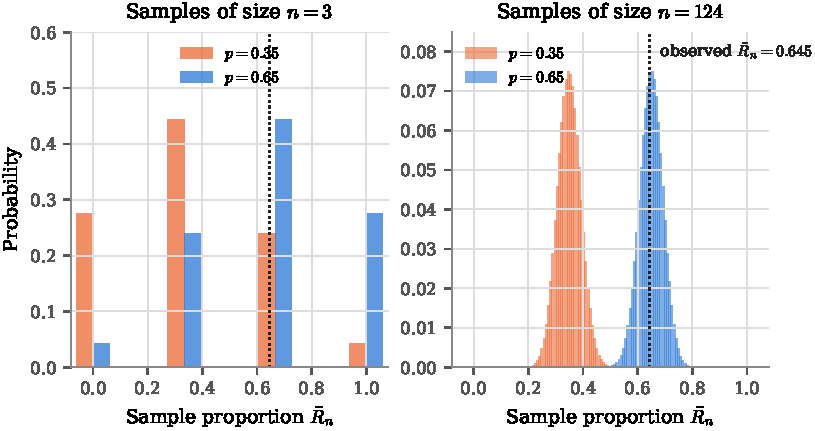
\includegraphics[width=\textwidth]{fig_kiss_samples}
\caption{What samples look like under two hypothetical truths. The bars are the exact (Binomial) distribution of the sample proportion $\bar{R}_n$ when the true proportion is $p = 0.35$ (orange) and when it is $p = 0.65$ (blue). With $n = 3$ (left) the two distributions overlap heavily: two or more right turns out of $3$ has probability $0.28$ under $p = 0.35$ and $0.72$ under $p = 0.65$, so three couples settle nothing. With $n = 124$ (right) the distributions have separated, and the observed $0.645$ (dotted line) is typical under $p = 0.65$ and essentially impossible under $p = 0.35$ (probability about $2 \times 10^{-11}$ of a proportion that large).}
\label{fig:kisssamples}
\end{figure}

The figure is the whole subject in miniature.
Under each candidate truth, probability tells you what the data would look like.
Statistics runs that backwards: the observed data are typical under some candidate truths and absurd under others, and the first group is your answer.
The rest of the book is about doing this with guarantees, and about doing it when the candidate truths form a continuum rather than two values.

\begin{bridge}[population, sample, parameter, statistic]
An introductory course describes a population (all kissing couples), a parameter of it ($p$, the proportion who turn right), a sample ($124$ couples) and a statistic computed from the sample ($\hat{p} = 0.645$) that estimates the parameter.
This book keeps all four words and changes what sits behind the first one.
The population is no longer a finite list of $5{,}000$ couples; it is a probability distribution, $\Bern(p)$, and a sample is $n$ independent draws from it.
The change is what makes the mathematics go: a finite population would make the draws slightly dependent (drawing without replacement) and would make the answer depend on the population size, while the distribution model gives clean results that hold whatever the size of the population and whether or not you can even list it.
\end{bridge}

Why does the model need probability?
Because you need to understand probabilistic aspects of the distribution of the random variable
\[
\hat{p} = \bar{R}_n = \frac{1}{n} \sum_{i=1}^n R_i.
\]
Specifically, you need to be able to answer questions such as:
\begin{itemize}[nosep]
\item Is the expected value of $\hat{p}$ close to the unknown $p$?
\item Does $\hat{p}$ take values close to $p$ with high probability?
\item Is the variance of $\hat{p}$ large? That is, does $\hat{p}$ fluctuate a lot?
\end{itemize}
Most of the probability tools needed are about averages of independent random variables, which is why Part II is about exactly that, once \cref{ch:models} has said what a model is.
For the kiss experiment the three answers are: $\E[\hat{p}] = p$ exactly; $\hat{p}$ is close to $p$ with high probability once $n$ is large (the Law of Large Numbers, \cref{ch:lln}); and $\var(\hat{p}) = p(1-p)/n$, which at $n = 124$ (and evaluated at $p = 0.645$, since $p$ itself is unknown) makes the typical fluctuation of $\hat{p}$ about $0.043$ (the Central Limit Theorem, \cref{ch:clt}, says the fluctuations are Gaussian).

\begin{pitfall}[is $64.5\%$ an estimator?]
No: $64.5\%$ is an estimate, and an estimate is not an estimator.
An \textbf{estimator} is a rule for turning data into a guess, $\hat{p} = \bar{R}_n$, and because the data are random the estimator is a random variable; it has an expectation, a variance and a distribution, and those are what \cref{fig:kisssamples} draws.
An \textbf{estimate} is the number the rule produced on the one sample you have, $\bar{r}_n = 0.645$.
It is one draw from the estimator's distribution: before the study, $\bar{R}_n$ could have come out anywhere from $0$ to $1$ with probabilities set by $p$, and the study produced one of those values.
Once observed it is a fixed number; the distribution belongs to the rule that produced it, not to the number.
Every statement about accuracy in this book is a statement about the estimator; the estimate is what you report.
\Cref{ch:lln} returns to this distinction under the name `theoretical sample mean', and \cref{sec:models-sample-space} walks the whole chain from the sample space to the number.
Outside that discussion and this box, the book follows the usual practice and writes the upper-case symbol with its realized value, $\bar{R}_n = 0.645$, trusting the context to say which of the two is meant.
\end{pitfall}

\section{The trinity of statistical inference}
\label{sec:kiss-trinity}

Everything statistical inference does falls under three headings, together called the trinity of statistical inference.
Here is each one as a sentence about the kiss experiment, with the chapter that makes the sentence precise.

\begin{enumerate}
\item \textbf{Estimation.} `$\hat{p} = \bar{R}_n$ is an estimator for the proportion $p$ of couples who turn their heads to the right.'
What makes it a good one? It is unbiased, its variance shrinks like $1/n$, and it is consistent.
\Cref{ch:estimators} defines these properties and compares estimators by them; \cref{ch:likelihood} shows that $\bar{R}_n$ is also the maximum likelihood estimator.

\item \textbf{Confidence intervals.} `$[0.56, 0.73]$ is a $95\%$ confidence interval for $p$.'
A range of truths under which the observed data are not surprising, with a guarantee about how often the procedure captures the truth.
\Cref{ch:confidence-intervals} builds this interval three ways and explains what the $95\%$ does and does not mean.

\item \textbf{Hypothesis testing.} `We find statistical evidence that more couples turn their heads to the right when kissing.'
A yes/no decision about $p$ with a controlled chance of being wrong.
\Cref{ch:tests-foundations} sets up the decision and \cref{ch:wald-lrt} supplies the general tests.
Here is the answer to the question of \cref{sec:kiss-test}: if the truth were $p = 1/2$, that is, if couples had no preference for either side, then the number turning right among $124$ couples would reach $72$ or more with probability $0.044$ and $75$ or more with probability $0.012$.
So $63$ right turns would be unremarkable (probability $0.46$ of at least that many), $72$ would be mild evidence, and $80$, which has probability $0.0008$ of being reached under $p = 1/2$, is strong evidence.
So $72$ is the threshold at the conventional $5\%$ level for this one-sided question; the two-sided version of \cref{ch:tests-foundations}, which also guards against $p < 1/2$, asks for $74$.
(Both numbers come from the exact Binomial distribution of the count; \cref{ch:tests-foundations} also derives the Gaussian-approximation versions, $72$ and $73$, and says why they can differ.)
\end{enumerate}

All three are statements about the same random variable $\bar{R}_n$, built from the same three modeling assumptions, and \cref{fig:trinity} draws them on one axis.
Change an assumption, for instance drop independence, and all three change.

\begin{figure}[htbp]
\centering
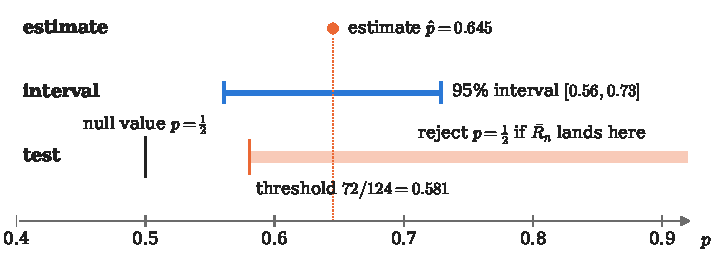
\includegraphics[width=\textwidth]{fig_trinity_axis}
\caption{The trinity on one axis. Every statement is about where $p$ sits on the line. The estimate is a point, $\hat{p} = 0.645$. The $95\%$ confidence interval is a bracket around it, $[0.56, 0.73]$: the truths under which the data are not surprising. The test compares the data to one particular truth, $p = \frac12$: if the observed proportion lands at or beyond the threshold $72/124 = 0.581$ (shaded), the data count as evidence against $p = \frac12$ and for $p > \frac12$. The threshold is set so that this happens only $5\%$ of the time when $p = \frac12$ really is the truth. \Cref{ch:confidence-intervals} and \cref{ch:tests-foundations} build the bracket and the threshold; the point is where both start.}
\label{fig:trinity}
\end{figure}

\section{What this book is and is not}
\label{sec:kiss-course}

This book has two aims: to introduce the mathematical theory behind statistical methods, and to supply theoretical guarantees for the methods you already use.
By the end you should be able to take a real-life situation like the kiss experiment, state it as a statistical problem in mathematical terms, choose methods appropriate to it, and say what those methods do and do not license you to conclude.
Four things recur throughout: the derivation of a standard method rather than its recipe, the justification of a quantitative statement from a stated set of modeling assumptions, the mathematics that arises in statistics and is worth seeing in its own right, and a toolbox of arguments that transfers to models the book never mentions.

Three things are outside its scope.
Applied modeling, meaning which data to collect and how to clean what you collected, is a separate subject, and the kiss experiment illustrates the point: \cref{sec:kiss-assumptions} takes the $124$ observations as given and says nothing about where and when to watch, or how to decide which way a pair of heads turned.
Implementation is not treated at all, and no formula here is tied to a particular piece of software.
And the aim is not a list of named methods: the general machinery of \cref{ch:wald-lrt} delivers whole families of tests at once, including most of the named ones, which is the reason for building it.
Where the undergraduate version of an idea makes the general version easier to see, that version appears in a box labeled `From undergraduate statistics'.

\section{What comes next}
\label{sec:kiss-next}

The three questions of \cref{sec:kiss-population} are all about the random variable $\hat{p} = \bar{R}_n$: its expectation, where it concentrates, how much it fluctuates.
The first has a one-line answer, $\E[\hat{p}] = p$.
Before any of them is answered, \cref{ch:models} turns the three assumptions of \cref{sec:kiss-assumptions} into an object, the statistical model, so that everything later can be stated for any model and not only this one.
The other two questions are about what happens as $n$ grows, and `as $n$ grows' is a limit, so Part II is about limits of random variables: \cref{ch:lln} says where $\bar{R}_n$ ends up, \cref{ch:clt} says what its fluctuations look like on the way, and \cref{ch:limit-tools} says what you may do to those limits (transform them, plug estimates into them) and still know where you are.
\Cref{ch:gaussian} then collects what you need about the Gaussian distribution, which is where all of the limits land.
If you are comfortable with limits of random variables already, \cref{ch:lln} opens with a box that says which parts of Part II are the minimal path.

\section{Summary}
\label{sec:kiss-summary}

\begin{itemize}[nosep]
\item Probability goes from a known mechanism to the data it produces; statistics goes from observed data back to the mechanisms that could have produced them. Same diagram, opposite arrows.
\item The kiss experiment: $n = 124$ couples, $80$ turned right, $\hat{p} = \bar{R}_n = 0.645$. It is the running example of the book.
\item Three modeling assumptions turn the data into mathematics: each $R_i$ is random, each is $\Bern(p)$ with the same $p$, and they are independent. Together: $R_1, \ldots, R_n \iid \Bern(p)$. Each assumption is a choice with a justification.
\item The population is a probability distribution, not a list; a sample is $n$ independent draws. The estimator $\hat{p}$ is a random variable; the estimate $0.645$ is one realization of it.
\item The trinity of inference: estimation (is $\hat{p}$ a good guess?), confidence intervals (which truths are compatible with the data?), hypothesis testing (is $p > 1/2$?). Every inferential method in this book is one of the three.
\end{itemize}

\section{Exercises}
\label{sec:kiss-exercises}

\begin{exercise}
Two dice are rolled and you win \$100 if you called the sum. Which total should you call, and what is your expected winning? Why is this a probability question rather than a statistics question?
\end{exercise}
\begin{solution}
Call $7$: six of the $36$ equally likely pairs sum to $7$, more than any other total, so the probability is $1/6$ and the expected winning is $100/6 \approx \$16.67$. The mechanism (fair, independent dice) is known in full, so there is nothing to learn from data; the answer is deduced.
\end{solution}

\begin{exercise}
In the drug example, verify the probability statement: if the drug cures each patient independently with probability $0.8$, show that the number cured out of $100$ has mean $80$ and standard deviation $4$, and explain why `at least $65$ cured' has probability very close to $1$.
\end{exercise}
\begin{solution}
The count is $\text{Bin}(100, 0.8)$ with mean $np = 80$ and standard deviation $\sqrt{np(1-p)} = \sqrt{16} = 4$. The value $65$ is $15/4 = 3.75$ standard deviations below the mean; a Gaussian approximation gives $\Pr(\text{at least } 65) \approx \Phi(3.75) \approx 0.9999$, and the exact Binomial computation gives $0.99985$.
\end{solution}

\begin{exercise}
Suppose the kiss data had been $n = 3$ couples, two turning right. Under the hypothetical truths $p = 0.35$ and $p = 0.65$, compute the probability of observing at least two right turns. What does the comparison tell you?
\end{exercise}
\begin{solution}
$\Pr(\text{at least } 2) = 3p^2(1-p) + p^3$, which is $0.282$ at $p = 0.35$ and $0.718$ at $p = 0.65$. The data are only about $2.5$ times more probable under the larger $p$, so three couples cannot distinguish the two truths; with $124$ couples the corresponding ratio is astronomically large (\cref{fig:kisssamples}).
\end{solution}

\begin{exercise}
Which of the three modeling assumptions would be violated in each case, and in which direction would it push $\hat{p}$? (a) The observer recorded each couple twice by mistake. (b) Half the couples were observed at a single wedding reception where the photographer told everyone to turn right. (c) The observer only recorded couples whose faces were visible from where the observer stood.
\end{exercise}
\begin{solution}
(a) Independence: the $124$ records are really $62$ independent observations, so $\hat{p}$ is as variable as a sample of $62$, not $124$, though its expectation is still $p$. (b) Identical distribution and independence: those couples share a $p_i$ near $1$ that is not the population's $p$, and they all followed the same instruction, so their outcomes are not independent; $\hat{p}$ is pushed upward. (c) The sample is not drawn from the population of interest at all: if being visible is related to the direction of the turn (it plausibly is, since from one side the observer sees the faces of couples who turn one way and the backs of the heads of couples who turn the other), the $R_i$ are Bernoulli with a parameter that differs from $p$, and no amount of data fixes it. The third is the most dangerous because it is invisible in the data.
\end{solution}
